%% LyX 2.3.7 created this file.  For more info, see http://www.lyx.org/.
%% Do not edit unless you really know what you are doing.
\documentclass[12pt,a4paper,preprint]{elsarticle}
\usepackage[latin9]{inputenc}
\usepackage{array}
\usepackage{float}
\usepackage{url}
\usepackage{amssymb}
\usepackage{graphicx}

\makeatletter

%%%%%%%%%%%%%%%%%%%%%%%%%%%%%% LyX specific LaTeX commands.
\pdfpageheight\paperheight
\pdfpagewidth\paperwidth

\DeclareTextSymbolDefault{\textquotedbl}{T1}
%% Because html converters don't know tabularnewline
\providecommand{\tabularnewline}{\\}

%%%%%%%%%%%%%%%%%%%%%%%%%%%%%% User specified LaTeX commands.
\usepackage{amssymb}
\usepackage{lineno}
\usepackage{url}
\journal{Softwarex}

\makeatother

\usepackage{listings}
\renewcommand{\lstlistingname}{Listing}

\begin{document}
\begin{frontmatter} 

\title{OPTIMUS: a multidimensional global optimization package  }

\author{Ioannis G. Tsoulos, Vasileios Charilogis, Alexandros Tzallas }

\address{Department of Informatics and Telecommunications, University of Ioannina, }
\begin{abstract}
A significant number of applications from many research areas can
be considered global optimization problems, such as applications in
the area of image processing, medical informatics, economic models,
etc. This paper presents a programming tool written in ANSI C++, which
researchers can use to formulate the problem to be solved and then
make use of the local and global optimization methods provided by
this tool to efficiently solve such problems. The main features of
the suggested software are: a) Coding of the objective problem in
a high level language such as ANSI C++ b) Incorporation of many global
optimization techniques to tackle the objective problem c)Parameterization
of global optimization methods using user-defined parameters.
\end{abstract}
\begin{keyword}
Global optimization\sep local optimization \sep stochastic methods
\sep evolutionary techniques\sep termination rules
\end{keyword}
\end{frontmatter}

\linenumbers

\section{Introduction }

The location of the global minimum for a continuous and differentiable
function $f:S\rightarrow R,S\subset R^{n}$ is formulated as
\begin{equation}
x^{*}=\mbox{arg}\min_{x\in S}f(x)\label{eq:eq1}
\end{equation}
where the set $S$ is defined as: 
\[
S=\left[a_{1},b_{1}\right]\otimes\left[a_{2},b_{2}\right]\otimes\ldots\left[a_{n},b_{n}\right]
\]
Methods that aim to locate the global minimum finds application in
problems from the area of economics \citep{globalecon1,globalecon2},
problems that appear very often in the area of physics \citep{global_physics1,global_physics2},
chemistry \citep{global_chemistry1,global_chemistry2}, common problems
from medicine \citep{global_med1,global_med2}, job scheduling problems
\citep{global_job1,global_job2}, water resources planning \citep{global_water1,global_water2},
network security problems \citep{global_network1,global_network2},
robotics \citep{global_robot1,global_robot2} etc. In the relevant
literature there are a number of global optimization techniques, such
as Adaptive Random Search methods \citep{go_adaptive1,go_adaptive2},
Controlled Random Search methods \citep{go_crs1,go_crs2}, Simulated
Annealing \citep{go_sa1,go_sa2,go_sa3}, Genetic algorithms \citep{go_ga1,go_ga2},
Ant Colony Optimization \citep{go_ant1,go_ant2}, Particle Swarm Optimization
\citep{go_pso1,go_pso2} etc. 

In this paper, a new integrated computing environment for performing
global optimization methods for multidimensional functions is suggested,
where the user can code the objective problem to ANSI C++. In addition
to the objective function, the programmer can also provide information
that the objective problem should have at the start of the optimization
process and, in addition, can formulate a series of actions that will
take place after the optimization process is finished. Similar software
environments can be found, such as the BARON software package \citep{baron}
, the MERLIN optimization software \citep{merlin} , the DEoptim software
\citep{deoptim} , the PDoublePop optimization software \citep{pdoublepop}
etc.

The rest of this article is structured as follows: in section \ref{sec:Method-description}
the proposed software is outlined in detail, in section \ref{sec:Experimental-results}
some experiments are conducted to show the effectiveness of the proposed
software and finally in section \ref{conclusions} some conclusions
and guidelines for future work are presented.

\section{Software description \label{sec:Method-description}}

\subsection{Distribution}

The suggested software is entirely coded in ANSI C++, using the freely
available QT programming library, which can be downloaded from \url{https://qt.io}
. At the present time, the software package can only be installed
on computers with the Linux operating system. The instructions to
install the package on a computer are as follows:
\begin{enumerate}
\item Download and install the QT programming library from \url{https://qt.io }. 
\item Download software from \url{https://github.com/itsoulos/OPTIMUS}.
\item Set the \emph{OPTIMUSPATH} environment variable pointing at the installation
directory of OPTIMUS e.g. OPTIMUSPATH=/home/user/OPTIMUS/, where user
is the user name in the Linux operating system. 
\item Set the \emph{LD\_LIBRAPY\_PATH} to include the OPTIMUS/lib subdirectory
e.g. \\
LD\_LIBRAPY\_PATH=\$LD\_LIBRAPY\_PATH:\$OPTIMUSPATH/lib/:
\item Issue the command: cd \$OPTIMUSPATH 
\item Execute the compilation script:\emph{ ./compile.sh }
\end{enumerate}
When the compilation is complete, the \emph{lib} folder will contain
the supported global optimization methods, the \emph{PROBLEMS} folder
will contain a number of example optimization problems from the relevant
literature, and the \emph{bin} folder will contain the main executable
of the software named \emph{OptimusApp}. 

\subsection{Implemented optimization methods }

In the proposed software, each implemented global optimization method
has a set of parameters that can determine the global optimization
path and the effectiveness of the method. The implemented global optimization
methods are:
\begin{enumerate}
\item Differential Evolution\citep{de_main_paper}, denoted as \textbf{de}. 
\item Improved Differential Evolution. The modified Differential Evolution
method as suggested by Charilogis et al \citep{gende} is implemented
and denoted as \textbf{gende}. 
\item Parallel Differential Evolution. A parallel implementation of the
Differential Evolution method as suggested in \citep{parallelDe}
is considered with the name \textbf{ParallelDe}.
\item A double precision genetic algorithm \citep{doublepop_tsoulos} is
included and it is denoted as \textbf{DoubleGenetic}.
\item Integer precision genetic algorithm. The method denoted as \textbf{IntegerGenetic}
is a copy of the \textbf{DoubleGenetic} method, but with the usage
of integer values as chromosomes.
\item Improved Controlled Random Search \citep{gcrs} is denoted as \textbf{gcrs}. 
\item Particle Swarm Optimization, denoted as \textbf{Pso}. 
\item Improved Particle Swarm Optimization, denoted as \textbf{iPso}, an
Particle Swarm method \citep{ipso}. 
\item Multistart. A simple method that initiates local searches from different
initial points is also implemented in the software. 
\item Topographical Multi level single linkage \citep{tmlsl} , denoted
as \textbf{Tmlsl}. 
\item The MinCenter method, denoted as \textbf{MinCenter} \citep{mincenter}.
\item NeuralMinimizer. A novel method that incorporates Radial Basis Functions
(RBF)\citep{rbf_main1} to create an estimation of the objective function
introduced in \citep{neuralMinimizer} is implemented and denoted
by the name \textbf{NeuralMinimizer}.
\end{enumerate}
Also, the parameter used to determine the used local optimization
procedure is the $--$localsearch\_method parameter and the implemented
methods are:
\begin{enumerate}
\item The \textbf{bfgs} method, denoting The Broyden--Fletcher--Goldfarb--Shanno
(BFGS) algorithm \citep{powell}.
\item The \textbf{lbfgs} method. The limited memory BFGS method \citep{lbfgs}.
\item The Gradient descent method, denoted as \textbf{gradient}.
\item The \textbf{adam} method. The adam local optimizer \citep{Adam} is
implemented also.
\item Hill climbing. The hill climbing local search procedure denoted as
\textbf{hill} is also implemented.
\end{enumerate}

\subsection{Objective problem deployment }

The objective problem must be coded in the C++ programming language.
Figure \ref{fig:A-typical-representation} shows an example of objective
function for the Rastrigin function. The implemented are as follows:
\begin{enumerate}
\item \textbf{void} init(QJsonObject data). The function init() is called
before the objective function is executed and its purpose is to pass
parameters from the execution environment to the objective function. 
\item \textbf{int} getDimension(), the dimension of the objective problem.
\item \textbf{void}    getmargins(vector\textless Interval\textgreater{}
\&x). The getmargins() functions returns in the vector x the bounds
of the objective problem. The class Interval is a simple class located
in the folder \emph{PROBLEMS} of the distribution, that represents
double precision intervals.
\item \textbf{double}	funmin(vector\textless\textbf{double}\textgreater{}
\&x). This function returns the objective problem $f(x)$ for a given
point $x$. 
\item \textbf{void}    granal(vector\textless\textbf{double}\textgreater{}
\&x,vector\textless\textbf{double}\textgreater{} \&g). This functions
stores in vector g the gradient $\nabla f(x)$ for a given point x.
\item QJsonObject  done(vector\textless\textbf{double}\textgreater{} \&x).
This function is executed after the objective function optimization
process is completed. The point x is the global minimum for the function
$f(x)$. 
\end{enumerate}

\subsubsection{Objective function compilation }

In order to build the objective function the user should create an
accompaniment project file as demonstrated in Figure \ref{fig:proFile}.
The software incorporates the utility qmake of the QT library to compile
the objective function. The compilation is performed with the following
series of commands in the terminal:
\begin{enumerate}
\item qmake \emph{file.pro}
\item make
\end{enumerate}
where\emph{ file.pro }stands for the name of the project file. The
final outcome of this compilation will be the shared library \emph{libfile.so}

\subsubsection{Objective function execution}

A full working command for the Rastrigin problem using the utility
program \emph{OptimusApp} is shown below

\begin{lstlisting}[language={C++},basicstyle={\normalsize},breaklines=true,literate={{-}{-}1}]
./OptimusApp --filename=librastrigin.so --opt_method=Pso\ --pso_particles=100 --pso_generations=10\  
    --localsearch_method=bfgs
\end{lstlisting}
The parameters for the above command line are as follows:
\begin{enumerate}
\item The argument of $--$filename determines the objective problem in
shared library format.
\item The argument of $--$opt\_method sets the used global optimization
procedure. 
\item The argument of $--$pso\_particles sets the number of particles of
the PSO optimizer.
\item The argument of $--$pso\_generations sets the maximum number of generations
allowed.
\item The argument of $--$localsearch\_method sets the used local optimization
procedure.
\end{enumerate}
The output of the previous command is shown in figure \ref{fig:rastrigin_output}. 

\section{Experiments \label{sec:Experimental-results}}

To assess the ability of the software package to adapt to different
problems, a series of experiments were performed under different conditions
and they are analyzed in the following subsections.

\subsection{Test functions}

To measure the effect of the proposed software, a series of experiments
were performed on test functions from the relevant literature \citep{testfunctions1,testfunctions2,testfunctions3,testfunctions4}.
The experiments were performed 30 times for every test case using
a different seed for the random number generator each time. Two variations
of the genetic algorithm (DoubleGenetic method) were used: one without
a local optimization method and one with periodic application of the
bfgs method at a rate of 5\% on the chromosomes in every generation.
The execution parameters for the genetic algorithm are listed in Table
\ref{tab:Experimental-settings} and the results are shown in Table
\ref{tab:results}. The numbers in parentheses show the percentage
of finding the global minimum, where the absence of this number denotes
that the algorithm discovered the global minimum in all executions.
The experimental results indicate that the usage of a local search
method in combination with the genetic algorithm significantly reduces
the required number of average function calls and also improves the
reliability of the method in finding the global minimum.

\subsection{The Lennard Jones potential}

The molecular conformation corresponding to the global minimum of
the energy of N atoms interacting via the Lennard-Jones potential
\citep{Jones,jonesNew} is used as a test case here. The function
to be minimized is given by:
\begin{equation}
V_{LJ}(r)=4\epsilon\left[\left(\frac{\sigma}{r}\right)^{12}-\left(\frac{\sigma}{r}\right)^{6}\right]\label{eq:potential}
\end{equation}
For testing purposes, the methods \textbf{NeuralMinimizer}, \textbf{DoubleGenetic}
and \textbf{Pso} was applied for a variety of numbers of atoms and
the results are shown in Table \ref{tab:potential}. The method NeuralMinimizer
requires a significantly reduced number of function calls compared
to the other two, while its reliability in finding the global minimum
for the potential remains high even when the number of atoms participating
in the potential increases significantly.

\subsection{Parallel optimization}

The High Conditioned Elliptic function, defined as 
\[
f(x)=\sum_{i=1}^{n}\left(10^{6}\right)^{\frac{i-1}{n-1}}x_{i}^{2}
\]
 is used as a test case to measure the scalability of the parallel
global optimization technique denoted as ParallelDe. This method was
applied to the problem with dimension increasing from 2 to 15 and
for a different number of processing threads. The experimental results
are shown in diagram form in Figure \ref{fig:Scalability} and they
indicate that the number of calls required to find the global minimum
decreases as the total processing threads increases, even though the
problem becomes increasingly difficult with increasing dimensions.

\section{Conclusions \label{conclusions}}

In this work, an environment for executing global optimization problems
was presented, where the user can code the objective problem using
some predefined functions and then has the possibility to choose one
among several global optimization methods to solve the mentioned problem.
This programming environment is freely available and easy to extend
to accommodate more global optimization techniques and it can be extended
in the near future with the following improvements:
\begin{enumerate}
\item Port the Optimums tool to other operating systems.
\item Use of modern parallel techniques to speed up the generated results. 
\item Implementing a GUI interface to control the optimization process.
\item The ability to code the objective function in other programming languages
such as Python, Ada, Fortran etc.
\item Creating a scripting language to efficiently guide the optimization
of objective functions.
\end{enumerate}
\begin{thebibliography}{999}
\bibitem{globalecon1} Zwe-Lee Gaing, Particle swarm optimization
to solving the economic dispatch considering the generator constraints,
IEEE Transactions on \textbf{18} Power Systems, pp. 1187-1195, 2003.

\bibitem{globalecon2}C. D. Maranas, I. P. Androulakis, C. A. Floudas,
A. J. Berger, J. M. Mulvey, Solving long-term financial planning problems
via global optimization, Journal of Economic Dynamics and Control
\textbf{21}, pp. 1405-1425, 1997.

\bibitem{global_physics1}Q. Duan, S. Sorooshian, V. Gupta, Effective
and efficient global optimization for conceptual rainfall-runoff models,
Water Resources Research \textbf{28}, pp. 1015-1031 , 1992.

\bibitem{global_physics2}P. Charbonneau, Genetic Algorithms in Astronomy
and Astrophysics, Astrophysical Journal Supplement \textbf{101}, p.
309, 1995

\bibitem{global_chemistry1}A. Liwo, J. Lee, D.R. Ripoll, J. Pillardy,
H. A. Scheraga, Protein structure prediction by global optimization
of a potential energy function, Biophysics \textbf{96}, pp. 5482-5485,
1999.

\bibitem{global_chemistry2}P.M. Pardalos, D. Shalloway, G. Xue, Optimization
methods for computing global minima of nonconvex potential energy
functions, Journal of Global Optimization \textbf{4}, pp. 117-133,
1994.

\bibitem{global_med1}Eva K. Lee, Large-Scale Optimization-Based Classification
Models in Medicine and Biology, Annals of Biomedical Engineering \textbf{35},
pp 1095-1109, 2007.

\bibitem{global_med2}Y. Cherruault, Global optimization in biology
and medicine, Mathematical and Computer Modelling \textbf{20}, pp.
119-132, 1994.

\bibitem{global_job1}Y. Gao, H. Rong, J.Z. Huang, Adaptive grid job
scheduling with genetic algorithms, Future Generation Computer Systems
\textbf{21}, pp. 151-161, 2005.

\bibitem{global_job2}D.Y. Sha, H.H. Lin, A multi-objective PSO for
job-shop scheduling problems, Expert Systems with Applications \textbf{37},
pp. 1065-1070, 2010.

\bibitem{global_water1}X. Cai, D.C. McKinney, L.S. Lasdon, Solving
nonlinear water management models using a combined genetic algorithm
and linear programming approach, Advances in Water Resources \textbf{24},
pp. 667-676, 2001.

\bibitem{global_water2}S.G. Gino Sophia, V. Ceronmani Sharmila, S.
Suchitra et al, Water management using genetic algorithm-based machine
learning, Soft Comput \textbf{24}, pp. 17153--17165, 2020.

\bibitem{global_network1}Z. Bankovic, D. Stepanovic, S. Bojanic,
O. Nieto - Taladriz, Improving network security using genetic algorithm
approach, Computers \& Electrical Engineering \textbf{33}, pp. 438-451,
2007.

\bibitem{global_network2}S. Paul, I. Dutt, S.N. Choudhri, Design
and implementation of network security using genetic algorithm. Int
J Res Eng Technol \textbf{2}, pp. 172-177, 2013.

\bibitem{global_robot1}A. Tuncer, M. Yildrim, Dynamic path planning
of mobile robots with improved genetic algorithm, Computers \& Electrical
Engineering \textbf{38}, pp. 1564-1572, 2012.

\bibitem{global_robot2}N. Kherici, Y.M. Ben Ali, Using PSO  for a
walk of a biped robot, Journal of Computational Science \textbf{5},
pp. 743-749, 2014.

\bibitem{go_adaptive1}M. Brunato, R. Battiti, RASH: A Self-adaptive
Random Search Method. In: Cotta, C., Sevaux, M., S�rensen, K. (eds)
Adaptive and Multilevel Metaheuristics. Studies in Computational Intelligence,
vol 136. Springer, Berlin, Heidelberg, 2008.

\bibitem{go_adaptive2}S. Andrad�ttir, A.A. Prudius, A.A., Adaptive
random search for continuous simulation optimization. Naval Research
Logistics \textbf{57}, pp. 583-604, 2010.

\bibitem{go_crs1}W.L. Price, Global optimization by controlled random
search, J Optim Theory Appl \textbf{40}, pp. 333--348, 1983.

\bibitem{go_crs2}P. Kaelo, M.M. Ali, Some Variants of the Controlled
Random Search Algorithm for Global Optimization. J Optim Theory Appl
\textbf{130}, pp. 253--264 (2006).

\bibitem{go_sa1}S. Kirkpatrick, C.D. Gelatt, M.P. Vecchi, Optimization
by simulated annealing, Science \textbf{220}, pp. 671-680, 1983.

\bibitem{go_sa2}K.M.El-Naggar, M.R. AlRashidi, M.F. AlHajri, A.K.
Al-Othman, Simulated Annealing algorithm for photovoltaic parameters
identification, Solar Energy \textbf{86}, pp. 266-274, 2012.

\bibitem{go_sa3}L.M. Rasdi Rere, M.I. Fanany, A.M. Arymurthy, Simulated
Annealing Algorithm for Deep Learning, Procedia Computer Science \textbf{72},
pp. 137-144, 2015.

\bibitem{go_ga1}J. Mc Call, Genetic algorithms for modelling and
optimisation, Journal of Computational and Applied Mathematics \textbf{184},
pp. 205-222, 2005.

\bibitem{go_ga2}C.K.H. Lee, A review of applications of genetic algorithms
in operations management, Elsevier Engineering Applications of Artificial
Intelligence \textbf{76}, pp. 1-12, 2018.

\bibitem{go_ant1}B. Chandra Mohan, R. Baskaran, A survey: Ant Colony
Optimization based recent research and implementation on several engineering
domain, Expert Systems with Applications \textbf{39}, pp. 4618-4627,
2012.

\bibitem{go_ant2}T. Liao, T. St�tzle, M.A. Montes de Oca, M. Dorigo,
A unified ant colony optimization algorithm for continuous optimization,
European Journal of Operational Research \textbf{234}, pp. 597-609,
2014.

\bibitem{go_pso1}D. Wang, D. Tan, L. Liu, Particle swarm optimization
algorithm: an overview. Soft Comput \textbf{22}, pp. 387--408, 2018.

\bibitem{go_pso2}N.K. Jain, U. Nangia, J. Jain, A Review of Particle
Swarm Optimization. J. Inst. Eng. India Ser. B \textbf{99}, pp. 407--411,
2018.

\bibitem{baron}N.V. Sahinidis, BARON: A general purpose global optimization
software package, J Glob Optim \textbf{8}, pp. 201--205, 1996.

\bibitem{merlin}D.G. Papageorgiou, I.N. Demetropoulos, I.E. Lagaris,
Computer Physics Communications \textbf{159}, pp. 70-71, 2004.

\bibitem{deoptim}K. Mullen, D. Ardia, D.L. Gil, D. Windover, J. Cline,
DEoptim: An R Package for Global Optimization by Differential Evolution,
Journal of Statistical Software \textbf{40}, pp. 1-26, 2011.

\bibitem{pdoublepop}I.G. Tsoulos, A. Tzallas, D. Tsalikakis, PDoublePop:
An implementation of parallel genetic algorithm for function optimization,
Computer Physics Communications \textbf{209}, pp. 183-189, 2016.

\bibitem{de_main_paper}R. Storn, On the usage of differential evolution
for function optimization, In: Proceedings of North American Fuzzy
Information Processing, pp. 519-523, 1996.

\bibitem{gende}V. Charilogis, I.G. Tsoulos, A. Tzallas, E. Karvounis,
Modifications for the Differential Evolution Algorithm, Symmetry \textbf{14},
447, 2022. 

\bibitem{parallelDe}V. Charilogis, I.G. Tsoulos, A Parallel Implementation
of the Differential Evolution Method, Analytics \textbf{2}, pp. 17-30,
2023.

\bibitem{openMp}R. Chandra, L. Dagum, D. Kohr, D. Maydan,J. McDonald
and R. Menon, Parallel Programming in OpenMP, Morgan Kaufmann Publishers
Inc., 2001.

\bibitem{doublepop_tsoulos}I.G. Tsoulos, Modifications of real code
genetic algorithm for global optimization, Applied Mathematics and
Computation \textbf{203}, pp. 598-607, 2008.

\bibitem{gcrs}V. Charilogis, I.G. Tsoulos, A. Tzallas, N. Anastasopoulos,
An Improved Controlled Random Search Method, Symmetry \textbf{13},
1981, 2021. 

\bibitem{ipso}V. Charilogis, I.G. Tsoulos, Toward an Ideal Particle
Swarm Optimizer for Multidimensional Functions, Information \textbf{13},
217, 2022.

\bibitem{tmlsl}M.M. Ali, C. Storey, Topographical multilevel single
linkage, J. Global Optimization \textbf{5}, pp. 349--358,1994

\bibitem{mincenter}V. Charilogis, I.G. Tsoulos, MinCentre: using
clustering in global optimisation, International Journal of Computational
Intelligence Studies \textbf{11}, pp. 24-35, 2022.

\bibitem{rbf_main1}J. Park, I.W. Sandberg, Approximation and Radial-Basis-Function
Networks, Neural Computation \textbf{5}, pp. 305-316, 1993.

\bibitem{neuralMinimizer}I.G. Tsoulos, A. Tzallas, E. Karvounis,
D. Tsalikakis, NeuralMinimizer, a novel method for global optimization
that incorporates machine learning, Information \textbf{14}, 2, 2023.

\bibitem{powell}M.J.D Powell, A Tolerant Algorithm for Linearly Constrained
Optimization Calculations, Mathematical Programming \textbf{45}, pp.
547-566, 1989. 

\bibitem{lbfgs}D.C. Liu, J. Nocedal, On the Limited Memory Method
for Large Scale Optimization, Mathematical Programming B \textbf{45},
pp. 503-528, 1989.

\bibitem{Adam}D.P. Kingma, J. Ba, Adam: A Method for Stochastic Optimization,
ICLR (Poster), 2015.

\bibitem{testfunctions1}M.M. Ali and P. Kaelo, Improved particle
swarm algorithms for global optimization, Applied Mathematics and
Computation \textbf{196}, pp. 578-593, 2008.

\bibitem{testfunctions2}H. Koyuncu, R. Ceylan, A PSO based approach:
Scout particle swarm algorithm for continuous global optimization
problems, Journal of Computational Design and Engineering \textbf{6},
pp. 129--142, 2019.

\bibitem{testfunctions3}Patrick Siarry, G�rard Berthiau, Fran�ois
Durdin, Jacques Haussy, ACM Transactions on Mathematical Software
\textbf{23}, pp 209--228, 1997.

\bibitem{testfunctions4}I.G. Tsoulos, I.E. Lagaris, GenMin: An enhanced
genetic algorithm for global optimization, Computer Physics Communications\textbf{
178, }pp. 843-851, 2008.

\bibitem{Jones}J.A. Northby, Structure and binding of Lennard-Jones
clusters: 13 \ensuremath{\le} n \ensuremath{\le} 147, J. Chem. Phys.
\textbf{87}, pp. 6166--6178, 1987.

\bibitem{jonesNew}G.L. Xue, R.S. Maier, J.B. Rosen, Improvements
on the Northby Algorithm for molecular conformation: Better solutions,
J. Global. Optim. 4, pp. 425--440, 1994.

\bibitem{ConPhysics}O.A. Sauer, D.M. Shepard, T.R. Mackie, Application
of constrained optimization to radiotherapy planning, Medical Physics
\textbf{26}, pp. 2359-2366, 1999.

\bibitem{ConAstro}F.P. Seelos, R.E. Arvidson, Bounded variable least
squares - application of a constrained optimization algorithm to the
analysis of TES Emissivity Spectra, in: 34th Annual Lunar and Planetary
Science Conference, March 17-21, 2003, League City, Texas, abstract
no.1817.

\bibitem{ConChem}M.J. Field, Constrained optimization of ab initio
and semiempirical Hartree-Fock wave functions using direct minimization
or simulated annealing , Journal of physical chemistry \textbf{95},
pp. 5104-5108, 1991.

\bibitem{ConBio}G.A. Williams, J.M. Dugan, R.B. Altman, Constrained
global optimization for estimating molecular structure from atomic
distances, Journal of Computational Biology \textbf{8}, pp. 523-547,
2001.

\bibitem{cons1}P.E. Gill, W. Murray, The computation of Lagrange-multiplier
estimates for constrained minimization, Mathematical Programming \textbf{17},
pp. 32-60, 1979.

\bibitem{cons2}M.J.D. Powell, Y. Yuan, A trust region algorithm for
equality constrained optimization, Mathematical Programming \textbf{49},
pp. 189-211, 2005.

\bibitem{cons3}K. Ichida, Constrained optimization using interval
analysis, Computers and Industrial Engineering \textbf{31}, pp. 933-937,
1996.

\bibitem{cons4}R.L. Becerra, C.A.C. Coello, Cultured differential
evolution for constrained optimization, Computer Methods in Applied
Mechanics and Engineering \textbf{195}, pp. 4303-4322, 2006.

\bibitem{Levy}A.V. Levy, A. Montalvo, The tunneling algorithm for
global optimization of functions, SIAM Journal of Scientific and Statistical
Computing \textbf{6}, pp. 15-29, 1985.

\bibitem{Salkin}H.M. Salkin, Integer programming, Edison Wesley Publishing
Com., Amsterdam, 1975.

\bibitem{Hess}R. Hess, A heuristic search for estimating a global
solution of non convex programming problems, Operations Research \textbf{21},
pp. 1267-1280, 1973.

\bibitem{choot}P. Chootinan, A. Chen, Constraint handling in genetic
algorithms using a gradient - based repair method, Computer and Operations
Research \textbf{33}, pp. 2263-2281, 2006.

\bibitem{G15}J.J. Liang, T.P. Runarsson, E. Mezura-Montes, M. Clerc,
P.N. Suganthan, C.A.C. Coello, K. Deb, Problem definitions and evaluation
criteria for the CEC2006 special session on constrained real-parameter
optimization, \url{http://www.ntu.edu.sg/home/EPNSugan/index_files/CEC-06/CEC06.htm}

\end{thebibliography}
\begin{figure}
\caption{A typical representation of an objective problem, suitable for the
OPTIMUS programming tool.\label{fig:A-typical-representation}}

\begin{lstlisting}[language={C++}]
# include <math.h> 
# include <interval.h> 
# include <vector> 
# include <stdio.h> 
# include <iostream> 
# include <QJsonObject> 
using namespace std;
extern "C" {
void    init(QJsonObject data) {
}
int	getdimension() { 	
	return 2; 
} 
void    getmargins(vector<Interval> &x) {         
  for(int i=0;i<x.size();i++)                 
	x[i]=Interval(-1,1); 
}
double	funmin(vector<double> &x) {    
	return (x[0]*x[0])+(x[1]*x[1])-cos(18.0*x[0])-cos(18.0*x[1]); 
}
void    granal(vector<double> &x,vector<double> &g) {       
	g[0]=2.0*x[0]+18.0*sin(18.0*x[0]);       
	g[1]=2.0*x[1]+18.0*sin(18.0*x[1]); 
}
QJsonObject    done(vector<double> &x) {     
return QJsonObject(); 
}
} 
\end{lstlisting}
\end{figure}
\begin{figure}
\caption{The associated project file for the Rastrigin problem.\label{fig:proFile}}

\begin{lstlisting}
TEMPLATE=lib 
SOURCES+=rastrigin.cc interval.cpp
HEADERS += interval.h
\end{lstlisting}
\end{figure}
\begin{figure}[H]
\caption{Output for the minimization of the Rastrigin function using the PSO
optimizer.\label{fig:rastrigin_output}}

\begin{lstlisting}
Generation     1 value:   -1.7464048
Generation     2 value:   -1.8619942
Generation     3 value:   -1.8852439
Generation     4 value:   -1.9490074
Generation     5 value:   -1.9490074
Generation     6 value:   -1.9490074
Generation     7 value:   -1.9490074
Generation     8 value:   -1.9775267
Generation     9 value:   -1.9972928
Generation    10 value:   -1.9977027
Minimum:       -2.0000000000  Function calls:    1028
\end{lstlisting}
\end{figure}
\begin{table}
\caption{Experimental settings\label{tab:Experimental-settings}}

\centering{}%
\begin{tabular}{>{\centering}p{0.49\textwidth}>{\centering}p{0.49\textwidth}}
\hline 
\textbf{PARAMETER} & \textbf{VALUE}\tabularnewline
\hline 
CHROMOSOMES & 200\tabularnewline
CROSSOVER RATE & 90\%\tabularnewline
MUTATION RATE & 5\%\tabularnewline
GENERATIONS & 200\tabularnewline
LOCAL SEARCH METHOD & bfgs\tabularnewline
\hline 
\end{tabular}
\end{table}

\begin{table}
\caption{Experimental results for some test functions using a series of global
optimization methods.\label{tab:results}}

\centering{}%
\begin{tabular}{>{\centering}p{0.33\textwidth}>{\centering}p{0.33\textwidth}>{\centering}p{0.33\textwidth}}
\hline 
\textbf{FUNCTION} & \textbf{GENETIC} & \textbf{GENETIC WITH LOCAL}\tabularnewline
\hline 
GRIEWANK2 & 9298(0.97) & 10684\tabularnewline
RASTRIGIN & 8967 & 11038\tabularnewline
SHEKEl5 & 19403(0.70) & 9222\tabularnewline
SHEKEL7 & 16376(0.80) & 8836\tabularnewline
SHEKEL10 & 19829(0.77) & 8729\tabularnewline
TEST2N4 & 17109 & 7786\tabularnewline
TEST2N5 & 19464 & 8264\tabularnewline
TEST2N6 & 24217 & 8868\tabularnewline
TEST2N7 & 26824 & 9376\tabularnewline
\textbf{SUM} & \textbf{161487(0.92)} & \textbf{82803}\tabularnewline
\hline 
\end{tabular}
\end{table}

\begin{table}[H]
\caption{Optimizing the Potential problem for different number of atoms.\label{tab:potential}}

\centering{}%
\begin{tabular}{>{\centering}p{0.24\textwidth}>{\centering}p{0.24\textwidth}>{\centering}p{0.24\textwidth}>{\centering}p{0.24\textwidth}}
\hline 
\textbf{ATOMS} & \textbf{GENETIC} & \textbf{PSO} & \textbf{NEURALMINIMIZER}\tabularnewline
\hline 
3 & 18902 & 9936 & 1192\tabularnewline
4 & 17806 & 12560 & 1964\tabularnewline
5 & 18477 & 12385 & 2399\tabularnewline
6 & 19069(0.20) & 9683 & 3198\tabularnewline
7 & 16390(0.33) & 10533(0.17) & 3311(0.97)\tabularnewline
8 & 15924(0.50) & 8053(0.50) & 3526\tabularnewline
9 & 15041(0.27) & 9276(0.17) & 4338\tabularnewline
10 & 14817(0.03) & 7548(0.17) & 5517(0.87)\tabularnewline
11 & 13885(0.03) & 6864(0.13) & 6588(0.80)\tabularnewline
12 & 14435(0.17) & 12182(0.07) & 7508(0.83)\tabularnewline
13 & 14457(0.07) & 10748(0.03) & 6717(0.77)\tabularnewline
14 & 13906(0.07) & 14235(0.13) & 6201(0.93)\tabularnewline
15 & 12832(0.10) & 12980(0.10) & 7802(0.90)\tabularnewline
\textbf{AVERAGE} & \textbf{205941(0.37)} & \textbf{137134(0.42)} & \textbf{60258(0.93)}\tabularnewline
\hline 
\end{tabular}
\end{table}
\begin{figure}[H]
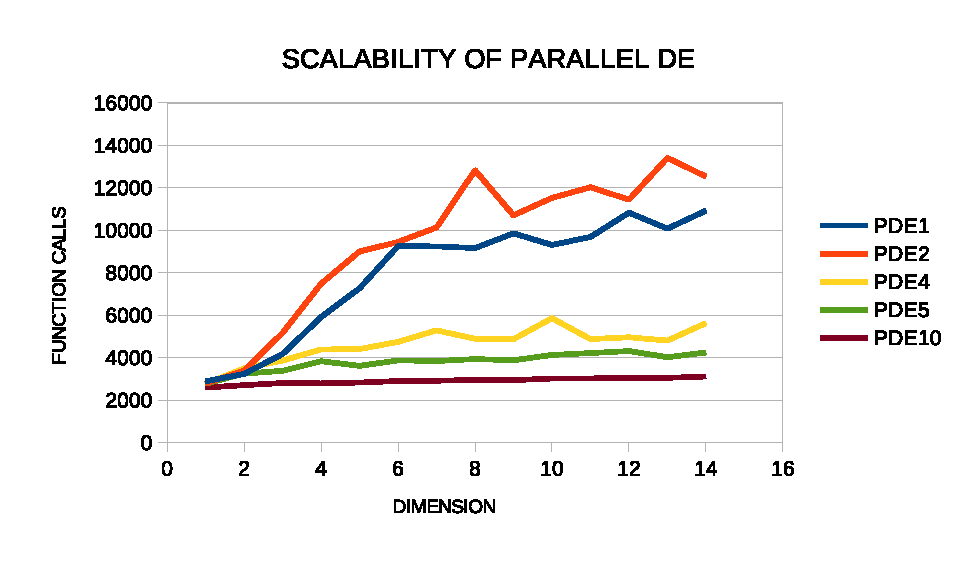
\includegraphics[scale=0.7]{parallelde_scale}

\caption{Scalabilty of the ParallelDe method.\label{fig:Scalability}}
\end{figure}


\section*{Required Metadata}

\label{}

\section*{Current code version}

\begin{table}[!h]
\begin{tabular}{|l|p{6.5cm}|p{6.5cm}|}
\hline 
\textbf{Nr.}  & \textbf{Code metadata description}  & \tabularnewline
\hline 
C1  & Current code version  & 1.0 \tabularnewline
\hline 
C2  & Permanent link to code/repository used for this code version  & \url{https://github.com/itsoulos/OPTIMUS/} \tabularnewline
\hline 
C3  & Legal Code License  & GNU General Public License (GPL) \tabularnewline
\hline 
C4  & Code versioning system used  & git \tabularnewline
\hline 
C5  & Software code languages, tools, and services used  & C++\tabularnewline
\hline 
C6  & Compilation requirements, operating environments \& dependencies  & Linux , QT Library\tabularnewline
\hline 
C7  & If available Link to developer documentation/manual  & \url{https://raw.githack.com/itsoulos/OPTIMUS/master/MANUAL/docs/html/index.html}\tabularnewline
\hline 
C8  & Support email for questions  & itsoulos@uoi.gr\tabularnewline
\hline 
\end{tabular}
\end{table}

\end{document}
